\section{Resisitive switch design}
\label{sec:resisitive_switch_design}
This chapter will show the theoretical concepts and propose a design of a cantilever based micro-switch.
Trade-offs and important parameters will be explained.
Also all simplifications are described here.

\subsection{Contact}
\label{sec:contact}
Optimized contact pads have serious constraints on geometry, materials, contact force and release force. 
Due to the small scope of this project the contact pads were not further studied and were defined as being of a simple rectangular shape.
The material was chosen to be gold for it's good electric and mechanical properties. 

A choice was made between two designs.
The first possibility was to use a cantilever with a single contact point, so that the current would flow through the cantilever itself. %image
The second possibility was to use a cantilever with a simple golden surface, that would connect two fixed contact points to one another. %image
The second design was chosen to guarantee a small lenght of the contact element and therefore to reduce it's resistance and power consumption.
Also the mechanical properties of the cantilever don't get influenced that heavily by the second choice and therefore enables the design, of all but the tip of the cantilever, to focus on the actuation and guidance functionality of the structure.
The disadvantage of this design choice is a minimum required width, which is given by the resolution of the fabrication process of two non-connected pads.
  
\begin{minipage}{\linewidth}
	\centering
	\begin{minipage}{0.35\linewidth}
		\begin{figure}[H]
	    	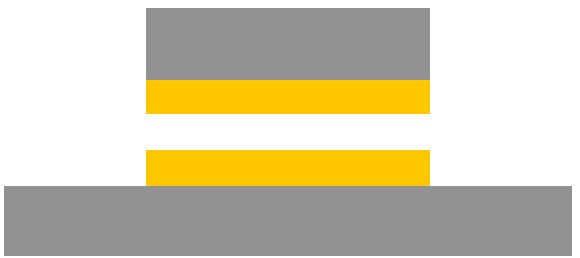
\includegraphics[width=\linewidth]{fig/cant_single_front.jpg}
	    	\caption{This is the first figure}
		\end{figure}
	\end{minipage}
	\hspace{0.05\linewidth}
	\begin{minipage}{0.35\linewidth}
		\begin{figure}[H]
	    	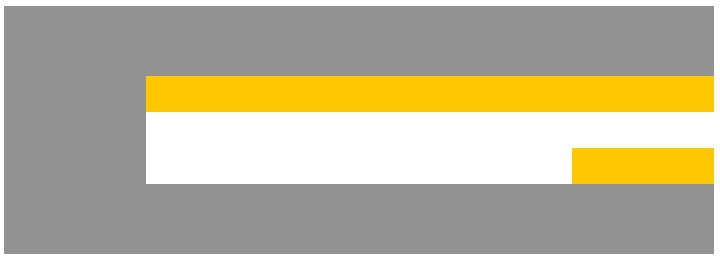
\includegraphics[width=\linewidth]{fig/cant_single_side.jpg}
	    	\caption{This is the second figure}
		\end{figure}
	\end{minipage}
\end{minipage}

\begin{figure}[h]
	\centering
	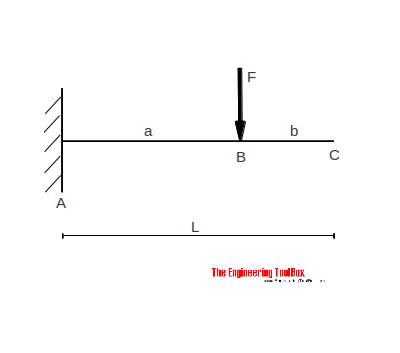
\includegraphics[width=8cm]{fig/cantilever_beam_single_load.png}
	\label{fig:cantilever_beam_single_load}
\end{figure}

\subsection{Actuation}
\label{sec:actuation}
There are four different actuation principles which can be used for a mechanical micro-switch design:
\begin{itemize}
  \item Electrostatic
  \item Piezoelectric
  \item Electromagnetic
  \item Thermal
\end{itemize}

Thermal actuators are not fast enough for micro-switch applications. 
Also they have the highest power consumption of all the methods.

Electromagnetic actuators require either a permanent magnetic material or an electromagnet design to work.
The material choices are therefore very difficult and also the footprint would be rather big compared to the other methods.

Piezoelectric actuators represent the method with the lowest power consumption.
But compared to electrostatic actuators they are way more complex to fabricate and material choices represent a huge challenge.\cite{klaasse2002piezoelectric}

Therefore our choice fell on an electrostatic actuator.
They are very simple from a fabrication point of view, allow low power consumption and offer a fast actuation time.

\subsection{Basic Concepts}
\label{sec:basic_concepts}


Area moment of inertia of recangular section:
\begin{equation}
	I_z = \frac{wt^3}{12}
	\label{eq:area_moment_of_inertia}
\end{equation}

Deflection of a beam:
\begin{figure}[h]
	\centering
	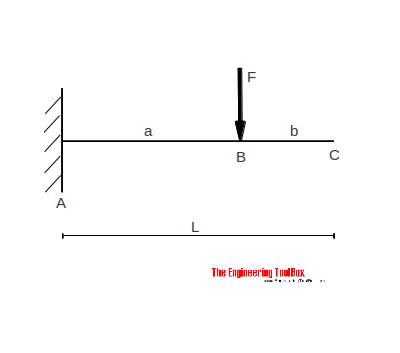
\includegraphics[width=8cm]{fig/cantilever_beam_single_load.png}
	\label{fig:cantilever_beam_single_load}
\end{figure}

\begin{equation}
	\delta_{max} = \frac{Fa^2}{6EI_z}\cdot(3l-a)
	\label{eq:beam_deflection}
\end{equation}

Effective mass:
\begin{equation}
	m_{eff} = \rho A \int_0^l{\left[\frac{\delta(x)}{\delta(l)_{max}}\right]^2dx} = \rho wt\frac{6l^2-4al+a^2}{12l-4a}
	\label{eq:effective_mass}
\end{equation}


- Frequency response / Minimal switching
Spring constant:
\begin{equation}
	k = \frac{F}{\delta} = \frac{6EI_z}{a^2(3l-a)}
	\label{eq:spring_constant}
\end{equation}

Resonance frequency:
\begin{equation}
	\omega_0 = \sqrt{\frac{k}{m_{eff}}}
	\label{eq:resonance_frequency}
\end{equation}

Capacitance actuator pad:
\begin{equation}
	C = \frac{\varepsilon A}{d}
	\label{eq:plate_capacitor}
\end{equation}

- Electrostatic analysis / Force <-> Area
Note: Distance smaller than surface, neglect fringes because of aspect ratio
\begin{equation}
	F_{ES} = \frac{\varepsilon AV^2}{2d^2}
	\label{eq:electrostatic_force}
\end{equation}

- Electric properties of contacts
Resistance:
mention asperity peaks
\begin{equation}
	R = \rho_{el}\frac{l}{wt}
	\label{eq:resistance}
\end{equation}

- Thermal
Not critical blablabla 

\subsection{Analysis}
\label{sec:analysis}
- Actuation point vs contact point placement
- Area contact
- Area actuator
- Beam cross section
- Material
